\documentclass{article}

\usepackage[main=english,vietnamese]{babel}
\usepackage[T1]{fontenc}
\usepackage[utf8]{inputenc}
\usepackage[sexy]{evan}
\usepackage{matchsticks}
\usepackage{wrapfig}
\usepackage{listings}

\newtheorem{hint}{Hint}

\title{Eight ways to prove - Part 1}
\author{Nghia Doan}
\date{\today}

\begin{document}

\maketitle

In this article, we explore different topics of geometry, each helps us to find a way for the same problem.

\begin{example*}[IMO 2014, Problem 4]
    Let $P$ and $Q$ be on segment $BC$ of an acute triangle $ABC$ such that $\angle PAB=\angle BCA, \angle CAQ=\angle ABC.$
    Let $M$ and $N$ be points on lines $AP$ and $AQ,$ respectively, such that $P$ and $Q$ are midpoints of $AM$ and $AN,$ respectively.
    Prove that the intersection $S$ of $BM$ and $CN$ is on the circumference of $\triangle ABC$.    
\end{example*}

\begin{proof}[\textbf{$1^{\text{st}}$ proof based on angle chasing and Cyclic Quadrilaterals}]

    First, $\angle PAB = \angle BCA = \angle C,$ and $\angle CAQ = \angle ABC = \angle B.$
    Thus $\triangle PBA \sim \triangle QAC \sim \triangle ABC.$

    \begin{center}
        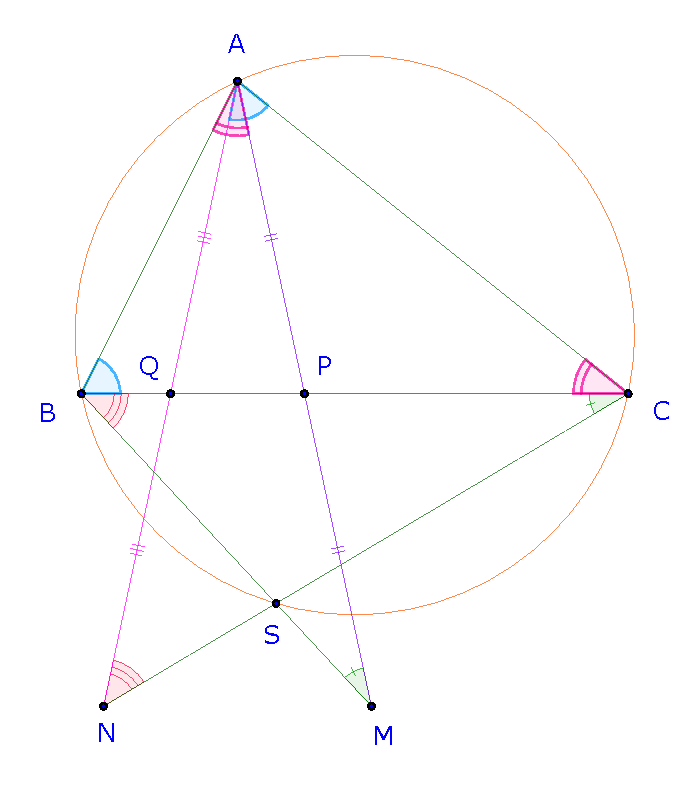
\includegraphics[width=8cm]{./svg/pdf/ot-22-23-4-e2-s1.pdf}
    \end{center}
    
    Thus, $\frac{PB}{PA} = \frac{QA}{QC},$ or $\frac{PB}{PM} = \frac{QN}{QC} \quad (1).$
     
    Now, $\angle BPM = \angle PAB + \angle PAB = \angle B + \angle C = \angle QAC + \angle QCA = \angle NQC \quad (2).$

    From (1) and (2) $\triangle BPM \sim \triangle NQC,$ so $\angle SBC = \angle MBP,\ \angle SCB = \angle NCQ.$

    Thus, $\triangle BSC \sim \triangle BPM,$ or $\angle BSC = \angle BPM = \angle B + \angle C = 180\dg  - \angle A.$

    Therefore $ABSC$ is cyclic and $S$ is on the circle $(ABC).$
\end{proof}

\newpage

\begin{proof}[\textbf{$2^{\text{nd}}$ proof based on similarity and Cyclic Quadrilaterals}]
    First, $\angle PAB = \angle BCA = \angle C,$ $\angle CAQ = \angle ABC = \angle B.$
    Thus $\triangle PBA \sim \triangle QAC \sim \triangle ABC.$

    Now, extend $AB$ and $AC$ to intersect line $MN$ at $Y$ and $Z,$ respectively.

    Since $Q, P$ are median segment, thus $MN \parallel BC.$
    Therefore $\triangle AMY \sim \triangle ABP \sim \triangle CAQ \sim \triangle ZAN.$

    $B$ is the midpoint of $AY$ in $\triangle AMY,$ $C$ is the midpoint of $ZA$ in $\triangle ZAN.$
    By similarity $\angle BNY = \angle CNA.$

    \begin{center}
        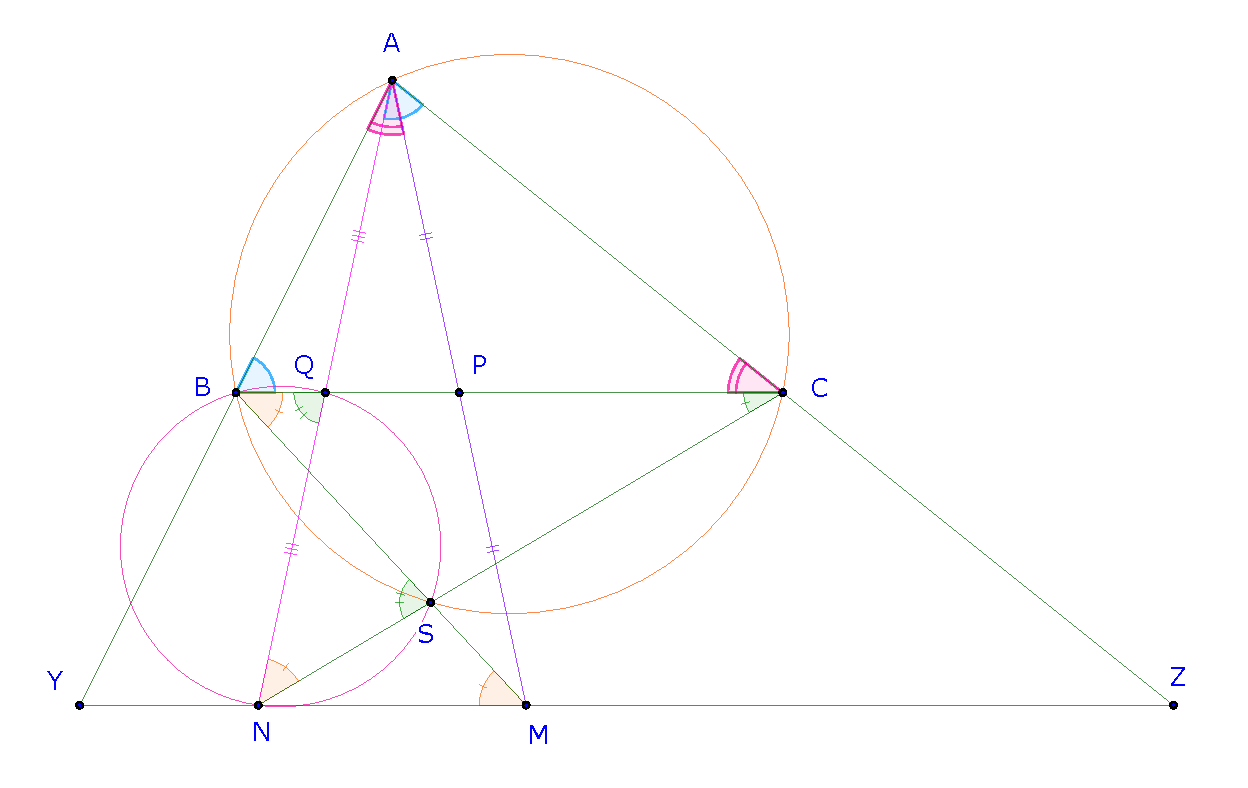
\includegraphics[width=14cm]{./svg/pdf/ot-22-23-4-e2-s5.pdf}
    \end{center}
    
    Therefore $\angle SBC = \angle BMN = \angle CNQ,$ so $BQSN$ is cyclic, thus $\angle NSB = \angle NQB = \angle CQA = \angle A.$

    Hence, $\angle BSC = 180\dg - \angle A,$ $ABSC$ is cyclic and $S$ is on the circle $(ABC).$
\end{proof}

\newpage

\begin{proof}[\textbf{$3^{\text{rd}}$ proof based on rigid transformations}]
    First, $\angle PAB = \angle BCA = \angle C,$ $\angle CAQ = \angle ABC = \angle B.$
    Thus $\triangle PBA \sim \triangle QAC \sim \triangle ABC,$
    \[
        \frac{AP}{AB} = \frac{AC}{BC},\ \frac{AQ}{AC} = \frac{AB}{BC} \Rightarrow AP = AQ.
    \]

    \begin{center}
        \begin{minipage}{8cm}
            \centering
            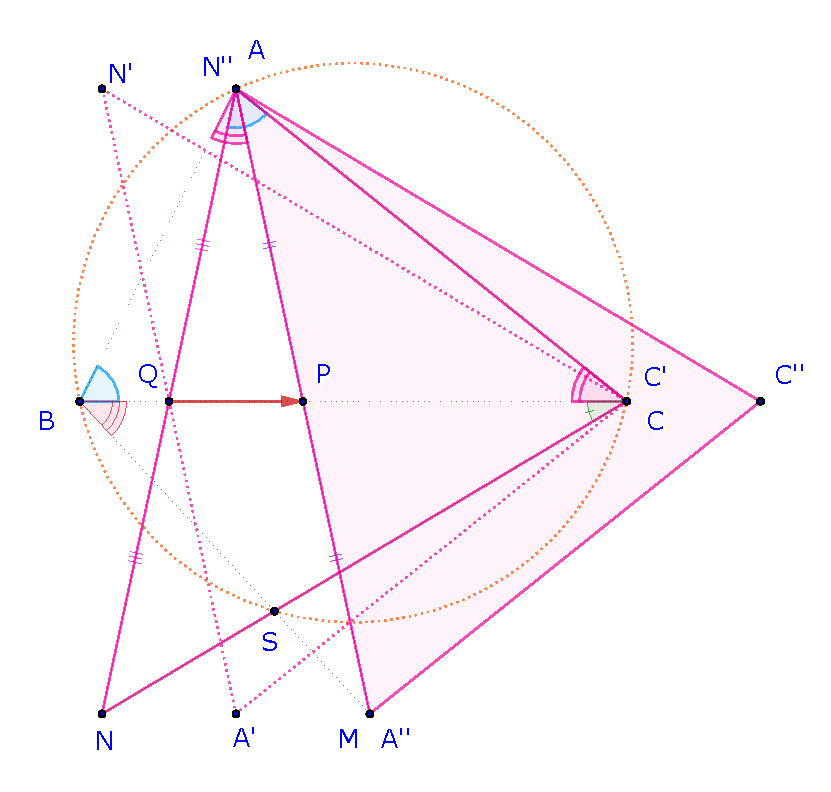
\includegraphics[width=8cm]{./svg/pdf/ot-22-23-4-e2-s6a.pdf}
        \end{minipage}
        \quad
        \begin{minipage}{8cm}
            \centering
            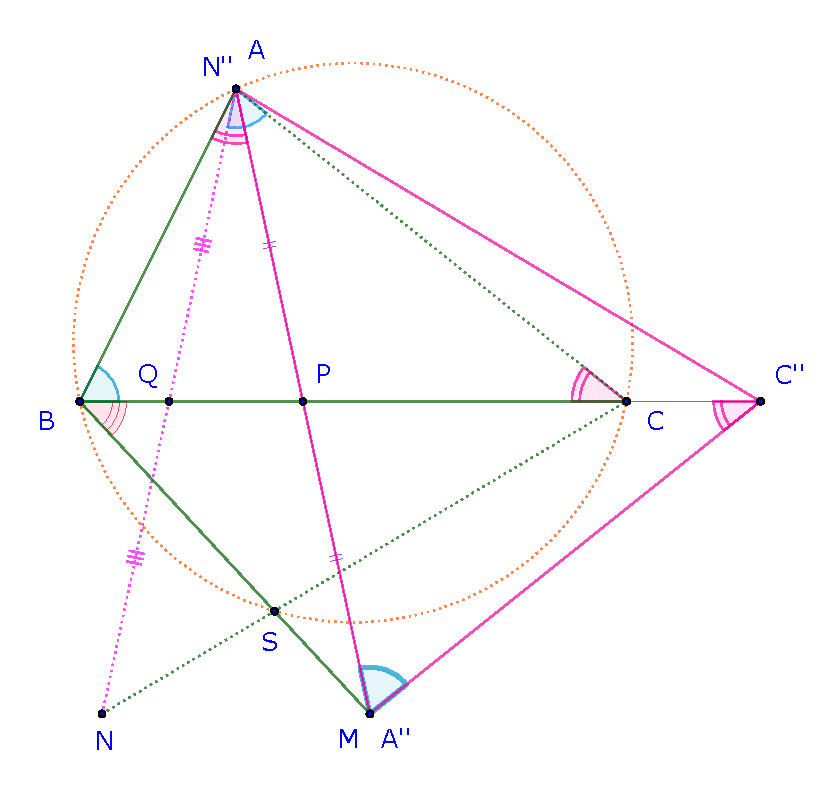
\includegraphics[width=8cm]{./svg/pdf/ot-22-23-4-e2-s6b.pdf}
        \end{minipage}
    \end{center}

    Thus, we can reflect the triangle $ANC$ over the line $BC$ to be $A'N'C',$
    then translate it by the vector $QP$ to be $A"N"C".$ Then segment $AM \equiv N"A".$

    $P$ is still the midpoint of $AM \equiv N"A",$ and $\angle BPA = \angle CQA = 180\dg - \angle C"PA.$
    Thus $C", C, P, Q, B$ are collinear.

    In quadrilateral $AC"A"B,$ $\angle C"BA = \angle C"A"A,$ thus it is cyclic, therefore $\angle A"BA + \angle A"C"A = 180\dg.$

    Thus $\angle ABS + \angle ACS = 180\dg.$ Therefore $ABSC$ is cyclic and $S$ is on the circle $(ABC).$
\end{proof}

\newpage

\begin{proof}[\textbf{$4^{\text{th}}$ proof based on Homothety}]
    Let $X$ and $Y$ be the midpoint of $AB$ and $AC,$ respectively.
    Let $Z$ be the intersection of $PX$ and $QY.$
    $\angle PAB = \angle BCA = \angle C,$ $\angle CAQ = \angle ABC = \angle B.$
    Thus $\triangle PBA \sim \triangle QAC,$ thus $\angle BXP = \angle AYQ.$
    Therefore $AXZY$ is cyclic.

    \begin{center}
        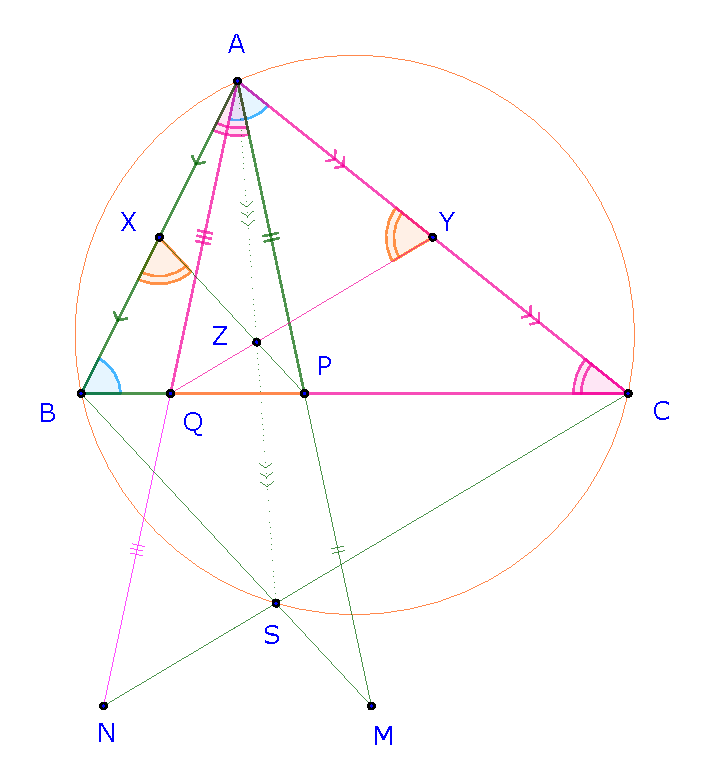
\includegraphics[width=7.5cm]{./svg/pdf/ot-22-23-4-e2-s2.pdf}
    \end{center}
    
    The homothety $\mathcal{H}_{(A, 2)}$ (center $A$ and factor $2$) sends $X, Y, P, Q$ to $B, C, M, N,$ respectively.

    $S = MB \cap NC$ ($MB \cap NC$ denotes the intersection of $MB$ and $NC$) thus it is the image of $PX \cap QY = Z.$

    $AXZY$ is cyclic. $ABSC$ is similar to $AXZY$ and therefore cyclic, too. Hence, $S$ is on circle $(ABC).$
\end{proof}

\end{document}